%% content.tex
%%

%% ===========================
\chapter{Konzeption}
\label{ch:Konzeption}
%% ===========================

Ein Konzept dient in der Softwarearchitektur der groben Strukturierung eines Softwaresystems. Zur Gestaltung werden neben funktionalen und nicht funktionalen Anforderungen, technische und organisatorische Einflussfaktoren hinzugezogen. Für erste Überlegung werden alle Komponenten, die zur Realisierung benötigt werden, in Verbindung zueinander gesetzt. Weiterhin sind Technologien festzulegen, die zur Umsetzung von bestimmten Komponenten verwendet werden können. Anschließend werden die Entwürfe, der einzelnen Komponenten im Detail beschrieben.  

%% ===========================
\section{Architektur}
%% ===========================

Zuerst wird ein erster Überblick über den groben Aufbau des Systems gegeben. In Abbildung \ref{konzept_architektur} können die Zusammenhänge des abzubildenden Software-Systems betrachtet werden. Bei einer Betrachtung in der 3-Schichten-Architektur stellt der Browser und die Client.war die Darstellungsschicht dar. Die Fachkonzeptschicht ist in der Server.war umgesetzt. Die Datenbank befindet sich zwar auch in der Server.war, allerdings ist sie trotzdem unabhängig und kann jederzeit separat betrieben werden.

\begin{figure}[htbp]
\centering
  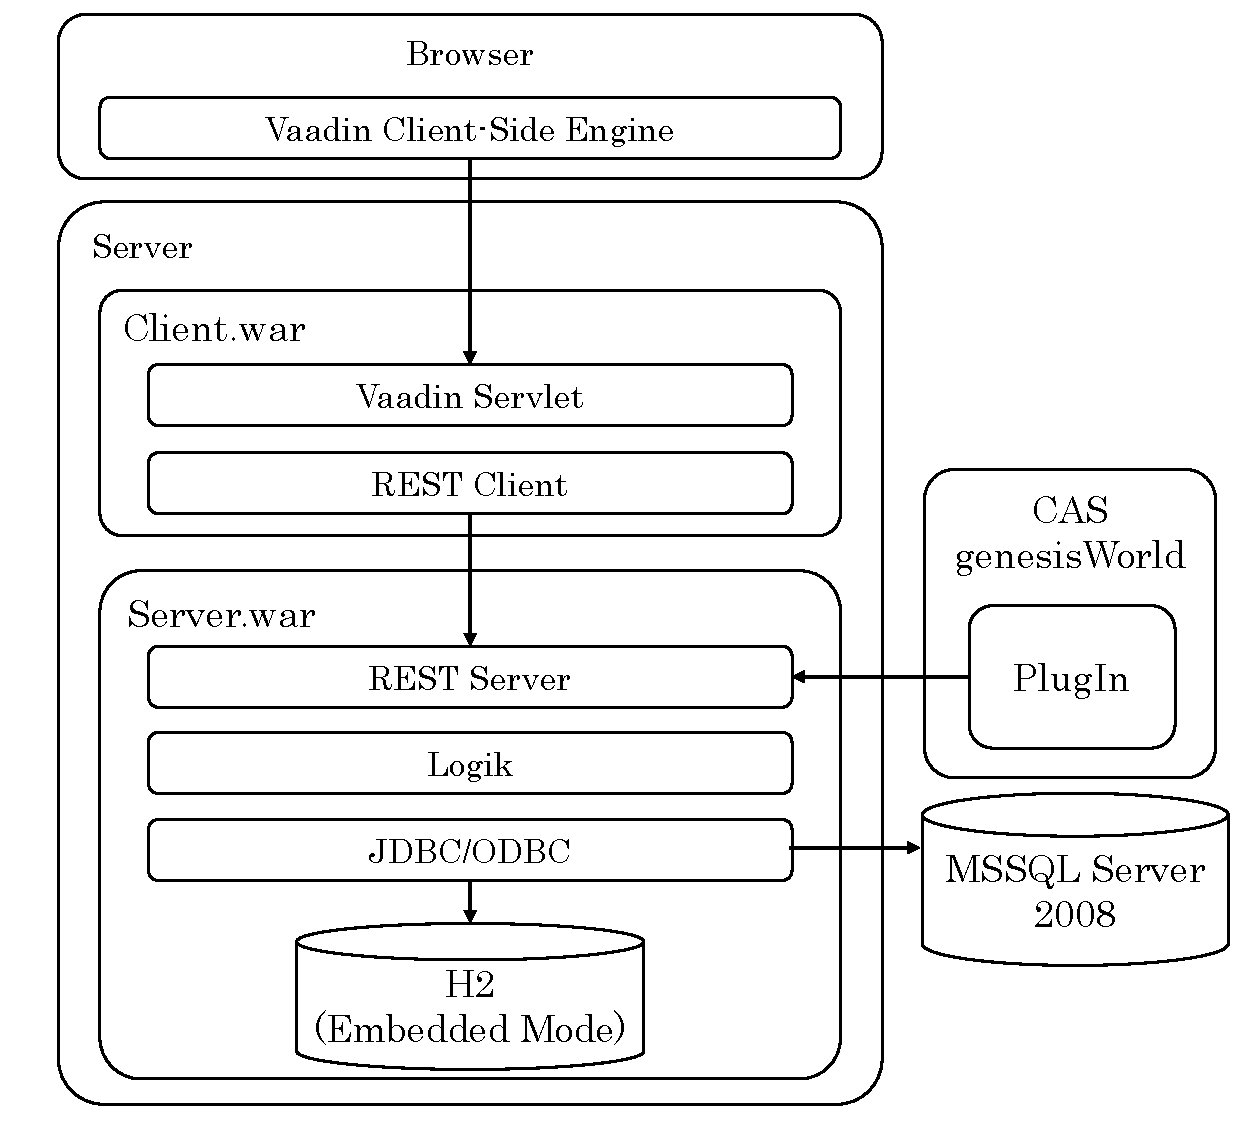
\includegraphics[width=0.8\textwidth, width=0.8\textwidth]{pics/Konzept_architektur.pdf}
\caption{Architektur des Systems}
\label{konzept_architektur}
\end{figure} 

Die Vaadin Client-Side Engine verwaltet das Rendering der Oberfläche im Web-Browser, durch den Einsatz verschiedener Client-Seitiger Widgets, die das Gegenstücke zu den serverseitigen Komponenten bilden. Es leitet Benutzerinteraktionen an die Server-Seite weiter und rendert anschließend die Änderungen für die Benutzeroberfläche. Die Kommunikation findet über asynchrone HTTP-oder HTTPS-Anfragen statt.

Server seitig arbeitet die Vaadin-Anwendungen auf der Java-Servlet-API. Das Vaadin Servlet oder genauer die VaadinServlet Klasse, ist für die Delegation verschiedenen Clients zuständig. Sie empfängt Anfragen und legt mithilfe von Cookies fest, welche Benutzersitzung zu welchem Client gehört.

Interaktion mit dem Benutzer-Interface-Komponenten erzeugen Events, die zunächst auf der Client-Seite durch Widgets verarbeitet werden. Nachfolgend werden die Events durch den HTTP-Server, das Vaadin Servlet und durch die Komponenten der Benutzeroberfläche geleitet, bis sie zu den in der Anwendung definierten Event-Listenern gelangen. In den Listenern wird mithilfe des REST-Clients ein POST-Requests an die Logik gesendet. Dieser enthält alle in der Oberfläche definierten Parameter. 

In der Server.war werden REST-Requests entgegen genommen. Anhand der mitübertragenen Filteroptionen, werden die Bedingungen für die Datenbank Abfrage zusammengestellt. Anschließend wird eine Verbindung zur H2-Datenbank aufgebaut. Das Ergebnis der Abfrage wird in das JSON-Format überführt und zurück an die Client.war geschickt. Dort angekommen werden die Daten an die Chart-Komponenten übergeben, was ein Neuaufbau der Komponente bewirkt.      

Eine der Anforderung ist die unabhängige Umsetzung von Client und Server. Der erste Schritt zur Umsetzung, der geforderten losen Kopplung zwischen Darstellung und Logik, wird durch die Aufsplittung in zwei verschiedene Anwendungen erreicht. Die Client.war beinhaltet die Klassen und Objekte der Darstellung. Wohingegen die Server.war alle Elemente zur Umsetzung der Logik beinhaltet. Die Verwendung des REST-Protokolls zwischen der Client.war und Server.war stellt den nächsten Schritt der losen Kopplung dar. Einer der Vorteile ist, dass Funktionen des Systems durch andere Clients abgegriffen werden können, ohne Änderungen am Server durchführen zu müssen. Beide WAR-Dateien werden in einem Apache Tomcat Webserver deployed und können über URLs angesprochen werden.

Die Logikkomponente in der Architektur stellt eine Zusammenfassung aller Funktionen des Anwendungskerns dar. Sie kümmert sich um die Generierung der Abfragen an die Datenbank. Welche eine dynamisch Generierung der Abfragen vornimmt, um nicht durch unnötigen Bedingungen, die Abfragegeschwindigkeit zu verringern. Abfragen werden mithilfe der Java Database Connectivity(JDBC) an die Datenbank gestellt. Neben der Generierung der Abfragen, enthält die Logikkomponente Funktionen zum Extrahieren und Transformieren der Daten aus der alten Datenbank. Der ETL-Prozess wird nur einmalig ausgeführt, allerdings stellt er einen der wichtigsten Schritte für die Umsetzung dar. 

Um nicht periodisch Extraktion und Transformation wiederholen zu müssen, wird ein selbstgeschriebenes PlugIn im CAS genesisWorld Anwendungsserver eingesetzt. Die Grundidee des PlugIns, ist Benachrichtigungen über Änderungen an unser System zu übermitteln. Dort wird Kontrolliert, ob der Datensatz eine Relevanz besitzt. Ist dies der Fall, besorgt sich die Anwendungslogik, anhand der zuvor übermittelten GGUID, alle benötigten Daten.

%% ===========================
\section{Technologien}
%% ===========================

Als einer der am meist verbreitetsten Programmiersprachen, stellt Java die Grundlage aller verwendeten Technologien dar. Zur Darstellung der Inhalte für den Client wird Vaadin verwendet. Der Apache Tomcat7 nimmt die Rolle des Anwendungsservers ein. Die Kommunikation auf Basis von RESTful Web Services wird mithilfe von Jersey realisiert. OpenSCV wird für das Lesen und Schreiben von CSV-Dateien verwendet. JDBC dient der Kommunikation zwischen Anwendungsserver und der Datenbank. Die H2-Datenbank stellt die Datenquelle des Systems dar. Im folgenden werden alle Bestandteile bis auf den H2 der bereits erläutert wurde, näher beschrieben. 

\paragraph{Vaadin}

Vaadin ist ein Open-Source-Java-basiertes Framework für den Aufbau von modernen Web-Anwendungen. Der Kerngedanke des Frameworks ist, dass alle Anwendungslogik in der Server-Seite ausgeführt wird, während die Client-Seite nur für das Senden der Benutzeraktionen an den Server und die Reaktion auf den Antworten, die er empfängt, verantwortlich ist. Da es auf GWT basiert, können sowohl die Client-und die Server-Code in reinem Java geschrieben werden.

Die aktuelle Version Vaadin , wurde im Februar 2013 veröffentlicht. Der bekannteste Wechsel von Vaadin 6, war die Integration von GWT zu Vaadin, die eine bessere Unterstützung für die clientseitige Widget Entwicklung bedeutete und sogar die Möglichkeit zu Erstellung von offline Vaadin-Anwendungen mit sich bringt.

Neben Open-Source, ist die im Unternehmen vorhandene Erfahrung, ein Grund für die Wahl des Frameworks. Ausschlaggebend war jedoch VaadinCharts, welches ein Erweiterung von Vaadin darstellt. Es basiert auf Highcharts, einem JavaScript-Packet, welches eine umfangreiche Sammlung an Funktionen zur Darstellung von Diagrammen besitzt. 

\paragraph{Jersey}

Jersey RESTful Web Services ist ein Open-Source-Framework zur Entwicklung von RESTful Web Services in Java, die Unterstützung für JAX-RS-APIs bietet und die JAX-RS (JSR 311 und JSR 339)-Referenzimplementierung darstellt. JAX-RS-Annotationen werden verwendet, um die REST Relevanz von Java-Klassen zu definieren. Jersey ist die Referenzimplementierung, der Spezifikation. Jersey enthält im Grunde einen REST-Server und einen REST-Client. Auf der Serverseite verwendet Jersey ein Servlet, die vordefinierten Klassen abtastet, um REST-Ressourcen zu identifizieren. Über die web.xml Konfigurationsdatei werden die von der Jersey-Distribution bereitgestellten Servlets registriert. Dieses Servlets analysieren die eingehenden HTTP-Anforderung und wählt die richtige Klasse und Methode für diese Anfrage aus. Diese Auswahl basiert auf Annotationen, in den Klasse und Methoden. Weiterhin unterstützt JAX-RS die Erstellung von XML-und JSON, über die Java Architektur für XML Binding (JAXB).

\paragraph{Apache Tomcat}

Tomcat ist ein Open-Source-Web-Server entwickelt von der Apache Group. Apache Tomcat implementiert die Java Servlet und der Javaserver Pages (JSP) Spezifikationen von Sun Microsystems und ist daher eine Referenzimplementierung. Er stellt weiterhin eine rein auf Java basierte HTTP Web Server Umgebung dar. Apache Tomcat enthält Tools für Konfiguration und Management, kann aber auch durch die Bearbeitung von XML-Dateien konfiguriert werden.

\paragraph{Opencsv}

Da Java das Parsen von CSV-Dateien nativ nicht unterstützt, müssen wir auf Drittanbieter-Bibliothek zurückgreifen. Opencsv ist eine sehr einfache CSV-Parser-Bibliothek für Java. Die Bibliothek kann zum erstellen, lesen und schreiben von CSV-Dateien benutzt werden. Die beste Fähigkeit des OpenCSV Parsers ist das Mapping von Ergebnissen auf Java-Bean-Objekte.

\paragraph{JDBC}

Die JDBC-API ermöglicht den programmgesteuerten Zugriff auf relationale Daten, aus der Java Programmiersprache heraus. Durch Verwendung der JDBC-API können Anwendungen SQL-Anweisungen ausführen, Ergebnisse abrufen und die Veränderungen auf die Datenquelle zurückschreiben. Der JDBC-API kann auch mit mehreren Datenquellen in einer verteilten, heterogenen Umgebung interagieren. 

%% ===========================
\section{Datenbankdesign}
%% ===========================

Das Datenbankdesign stellt einen der wichtigsten Abschnitte der Konzeption dar. Festlegungen im Bereich des Datenmodells werden in dieser Phase getroffen. Sie entscheiden ob Anforderungen und Erwartungen erfüllt werden können. In dieser Phase sind die Charakteristika der Daten zu untersuchen und das Datenmodell entsprechend nach ihnen auszulegen.

%% ===========================
\subsection{Konzeptionelles Design}
%% ===========================

Normalisierung dient der Organisation von Feldern und Tabellen einer relationalen Datenbank, um Redundanz und Abhängigkeit zu minimieren. Die Kehrseite hingegen ist eine Steigerung des Aufwands, um die benötigten Daten wiederzugewinnen. Normalisierung bietet die Möglichkeit einen Austausch zwischen Performance und Stabilität des Datenbankmodells vorzunehmen. 
In unserem Fall stellt ersteres absolute Priorität dar. Daher wird versucht, die Normalisierung so gering wie möglich zu halten. 

Die erste Überlegung hinsichtlich des Schemas ist, welche Daten für die Beantwortung der Abfragen benötigt werden. Der Datenbankdesigner steht bei analytischen System immer vor der Entscheidung, wie viele Information aus dem alten System in das Neue übernommen werden sollten. Um höchst mögliche Performance zu erreichen werden lediglich die für das Szenario benötigten Daten extrahiert. Allerdings entsteht durch nachträgliche Hinzunahme von Funktionen ein erhöhter Aufwand für Änderungen am Schema und des ETL-Prozesses. Abbildung \ref{konzept_SchemaNeu} zeigt das für die Datenbank neu entworfene Schema. 

\begin{figure}[htbp]
\centering
  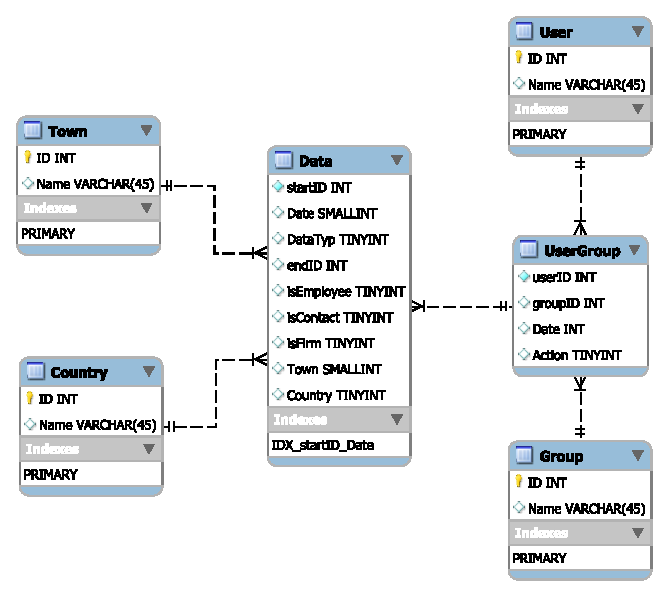
\includegraphics[width=0.8\textwidth, width=0.8\textwidth]{pics/NewSchema.pdf}
\caption{Neue Datenbankschema}
\label{konzept_SchemaNeu}
\end{figure} 

Die Idee hinter dem Schema ist, die Verwendung einer einzelnen Tabelle zur Aufbewahrung der Informationen, der Verbindungsmerkmale. Diese Tabelle ermöglicht es, ausgehend von einem Benutzer, alle Verbindungen zu anderen Personen zu finden. Im Grunde genommen sind vier Spalten dafür ausreichend. Die erste Spalte startID beinhaltet die Person, von der die Suche ausgeht. Eine Zuordnung der Tupel zu einem Datum erfolgt über die Spalte Date. Um Verbindungsmerkmale zu unterscheiden, wird der Typ in der Spalte DataTyp vermerkt. Die letzte Spalte endID beinhaltet die Personen zu denen die Verbindungsmerkmale letztendlich führen. Anderen Spalten wie z.B. Town oder Country dienen lediglich der Filterung der Ergebnisse.

Um mit den geringeren Speicherkapazitäten die uns zur Verfügung stehen zurechtzukommen, wird auf das Problem der Datenredundanz eingegangen. Durch Normalisierung lässt sich Datenredundanz zwar nicht verringern, allerdings kann man sie in kontrollierbare Bahnen lenken. Im neuen Schema wurden solche Maßnahmen auf die Spalte Town und Country angewendet. Beide Spalten werden voraussichtlich Millionen von Werten beinhalten. Es gibt jedoch nur 193 Länder auf der Welt. Das bedeutet das Wörter, wie Deutschland sich sehr oft wiederholen. Die Spalte Country ist vom Datentyp Varchar, welches pro Zeichen 2 Byte benötigt. Das wären beim Wort Deutschland 22 Byte. Legt man nun für die Spalte Country eine neue Tabelle an, wird in dieser jedes Land nur einmal vermerkt. Jedes Land bekommt einen Schlüssel in Form einer Zahl. In der eigentlichen Tabelle Data werden nur noch die Zahlen, anstatt des vollständig ausgeschrieben Wortes, verwendet. Das würde beispielsweise mit dem Wort Deutschland eine Reduktion von 22 Byte auf 1 Byte bewirken. Die Reduzierung auf 1 Byte lassen sich auf das TINYINT Format zurückführen. Das gleiche gilt für die Spalte Town. Bei ihr wird allerdings der Datentyp SMALLINT verwendet, mithilfe dessen ein Zahlenbereich von -32768 bis 32767 abgebildet werden kann. Die Spalten isEmployee, isContact und isFirm können nur zwei verschiedene Zustände darstellen. Stimmt oder stimmt nicht. Der Datentyp TINYINT reicht daher zur Abbildung des Zustandes völlig aus. Ein Feld vom Typ datetime benötigt 8 byte an Speicher. Um hier ebenfalls Einsparungen vorzunehmen, wurde beschlossen das Datum als SMALLINT zu deklarieren. Dies ist möglich da nur das Tages-Format des Datums von Interesse ist. Dazu wird ein frei gewählter Nullpunkt festgelegt. In unserem Fall wurde der 01.01.1990 als Nullpunkt gewählt, da keine älteren Daten existieren. Darauf aufbauend wird das Datum, durch die Differenz in Tagen zum Nullpunkt, in der Spalte Date abgelegt. Die Hochrechnung der Tabelle \ref{tb_speicherplatzverbrauch} zeigt, dass durch die Normalisierung der Speicherplatzverbrauch um den Faktor 6 gesenkt werden kann.

\begin{table}[htbp]
\centering
\begin{tabulary} {\linewidth} {l  r  C  l  C  r}
& & & & & \\
\multicolumn{6}{l}{Speicherplatzverbrauch ohne Normalisierung}\\
& & & & & \\
Zeitpunkt(timestamp) & 8 byte & x & 18.000.000 & = & \textasciitilde 137 MB \\  
Stadt(varchar) & 16 byte & x & 18.000.000 & = & \textasciitilde 343 MB \\  
Land(varchar) & 20 byte & x & 18.000.000 & = & \textasciitilde 274 MB \\  
\midrule
& & & & Summe & \textasciitilde 754 MB\\
& & & & & \\
\multicolumn{6}{l}{Speicherplatzverbrauch mit Normalisierung}\\
& & & & & \\
Zeitpunkt(smallint) & 2 byte & x & 18.000.000 & = & \textasciitilde 34 MB \\  
Stadt(integer) & 4 byte & x & 18.000.000 & = & \textasciitilde 72 MB \\  
Stadt(varchar) & 16 byte & x & 21.000 & = & \textasciitilde 0,32 MB \\  
Land(tinyint) & 1 byte & x & 18.000.000 & = & \textasciitilde 17 MB \\  
Land(varchar) & 20 byte & x & 218 & = & \textasciitilde 0,004 MB \\
\midrule  
& & & & Summe & \textasciitilde 123 MB\\
& & & & & \\
\end{tabulary}
\caption{Vergleich des Speicherplatzverbrauchs}
\label{tb_speicherplatzverbrauch}
\end{table}

Möchte man nun die Abfrage eines Benutzers, die eine Filterung anhand einer Stadt voraussieht beantworten, muss man zuerst an die ID der Stadt herankommen. Dabei können zwei verschiedene Ansätze verfolgt werden. Der erste Ansatz wäre einen Join zwischen Town und Data, um direkt mit dem Namen der Stadt zu arbeiten. Diese Variante dürfte aufgrund des Kreuzproduktes von Millionen von Zeilen nicht sehr performant sein. Eine andere Möglichkeit ist, eine separate Abfrage an die Datenbank zu stellen, in der die ID zum Namen ermittelt wird. Mithilfe der ID kann dann ohne einen Join die Ergebnismenge ermittelt werden. Dieser Ansatz dürfte vor allem durch die Abwesenheit von Netzwerkzugriffen zur besseren Performance führen. Dieses Vorgehen kann für die Stadt, das Land und die Gruppenzugehörigkeit angewendet werden.

Die Tabelle GroupDate unterscheidet sich von den anderen Auslagerungstabellen, den dort sind noch weitere Details vermerkt. Diese ermöglichen es die Zusammenstellung von Gruppen über die Zeit nachzuvollziehen. Action legt fest ob die Tupel einen Eintritt einer Person oder einen Austritt darstellt. Die Spalte Date beinhaltet das Datum, des Ereignisses. Mithilfe beider Attribute lassen sich Gruppenzusammenätzungen auf bestimmte Zeitpunkte bezogen rekonstruieren.

%% ===========================
\subsection{Zugriffsstrukturen}
%% ===========================

Indizes dienen der Beschleunigung von Suchen nach bestimmten Spaltenwerten. Ohne Indexe müsste die H2-Datenbank beim ersten Datensatz beginnen und dann die gesamte Tabelle durchgehen, um eine Abfrage zu beantworten. Je größer die Tabelle ist, desto höher sind die Kosten dafür. Daher bietet der Einsatz sich gerade in Anbetracht nach der Forderung von Performance an. Zu Beachten ist jedoch, dass jeder Index einen Zuwachs des Speicherplatzverbrauchs mit sich bringt. Zur Indexierung der Tabellen Town, Country, User und Group eignen sich Hash-Indizes. Sie bieten einen extrem schnellen Zugriff auf die Daten. Diese Schnelligkeit ergibt sich aus der Verwendung von Berechnungsvorschriften, zur Ermittlung der Position, des gesuchten Wertes. Indiziert werden in unserem Schema die Spalte Name in der jeweiligen Tabelle, da der Client nur die jeweiligen Namen besitzt. Mithilfe der Namen werden die zugehörigen IDs ermittelt. Die Nutzung von Hash-Indizes bringt allerdings Limitierungen mit sich. Eine der wichtigsten ist, dass Sie nur für Vergleiche("=") verwendet werden können. Somit werden keine Wertebereich-Abfragen("<" oder ">") unterstützt. Es gibt allerdings noch andere Nachteile \cite{SWB-352401869}, auf die aber in dieser Arbeit nicht näher eingegangen wird. 
Für die Tabelle UserGroup eignet sich der Standard Index von H2, der ein B\textsuperscript{+}-Baum verwendet. Dieser kann für die Spalte userID verwendet werden, der den ersten Wert einer Suche darstellt. Der B\textsuperscript{+}-Baum eignet sich auch für die Data-Tabelle. Hier ist außerdem die Verwendung eines Mehr-Attribut-Indexes vorgesehen. Der Vorteil eines Mehr-Attribut-Indexes ist, dass bei einer Punkt-Abfrage über alle Zugriffsattributwerte nur ein Indexzugriff erfolgen muss. Indexiert werden in unserem Fall die Spalte startID und Date. Beide Spalten sind sortiert und bieten sich somit für die Verwendung eines geclusterten Index an. Geclusterte Indizes sind in der gleichen Form sortiert wie die interne Relation. Ein geclusterter Index unterstützt Bereichsanfragen sehr gut, was bei der Beschränkung auf Zeitspannen von Vorteil sein dürfte.       


%% ===========================
\section{Extract Transform Load Prozess}
%% ===========================

Daten der operativen Systeme unterstützen die wertschöpfende Geschäftsprozesse innerhalb eines Unternehmens. Sie sind demnach auf die Steuerung und Überwachung des Tagesgeschäftes ausgerichtet und daher transaktionsbezogen. Somit sind die Daten in Ihren Begrifflichkeiten häufig nicht vergleichbar und ihrer Bewertung sowie Konsolidierung unterschiedlich. Um die Daten dennoch für analytische Zwecke einzusetzen, ist eine Überführung in eine geeigneter Struktur von Vorteil. Eine solche Überführung wird in der Literatur als Extract, Transform, Load (ETL)-Prozess bezeichnet \cite{ElSappagh201191}. 

%% ===========================
\subsection{Extract}
%% ===========================

Zunächst dient die Extraktion primär der Beschaffung von Daten aus dem MSSQL Server 2008. Überdies können durch den Prozess Daten bereits reduziert,  zusammengeführt und ersetzt werden. Für eine zutreffende Formulierung der Abfragen, müssen Besonderheiten in die Ermittlung der Daten beachtet werden. Eine vollständige und korrekte Datenmenge stellt die Grundlage jeder guten Analyse dar.

Die erste Besonderheit stellt die Betrachtung in Bezug auf Zeitspannen dar. Bei Analysen über die Zeit ist zu beachten, dass Daten sich im Laufe der Zeit verändern und dies zu berücksichtigen ist. Die Tabelle Changelogbook bietet uns die Möglichkeit, Veränderungen in den Datensätzen nach zu vollziehen. Eine solche Veränderungen über die Zeit, ist in der Gruppenkonstellation zu finden, da Personen Gruppen verlassen oder beitreten können. Neben den Veränderungen über die Zeit sind Datensätze, die über mehrere Tage gehen, gesondert zu behandeln. Termine wie Tagungen und der gleichen erstrecken sich beispielsweise über mehrere Tage. In der MSSQL Datenbank werden diese Termine als ein Datensatz beachtet. In unserer Analyse stellt jede Tupel eine Verbindung dar. Jede Tupel besitzt einen Tag der für die Analyse herangezogen wird. Somit muss ein Datensatz, der sich über mehrere Tage erstreckt, in der H2-Datenbank durch mehrere Tupeln repräsentiert werden. Deswegen sollte im Ergebnis der SQL-Query vermerkt werden, dass dieser Termin mehrere Tage ging, damit dies in der Transformation berücksichtigt werden kann. 

Eine weitere Besonderheit ergibt sich, durch ein nicht im System vorgesehenes Verhalten der Benutzer, welche die Auswertung der Daten erschwert. CAS genesisWorld ermöglicht es Termine zu schieben. Diese Funktion wird von manchen Nutzern missbraucht. Anstatt für einen ähnlichen Termin einen neuen Eintrag anzulegen, wird ein alter aus Bequemlichkeit geschoben. Das hat zur Folge, dass Termine die tatsächlich statt gefunden haben, in der Datenbank nicht mehr existieren. Um trotzdem diese Termine zu berücksichtigen wurde folgendes Konzept erarbeitet. Dem Changelogbook lässt sich entnehmen, ob die Feld start\_dt und end\_dt verändert wurden. Zur Feststellung ob ein Termin stattgefunden hat und anschließend geschoben wurde, müssen zwei Bedienungen erfüllt sein. Die erste ist, dass der Termin nach dem angegeben Zeitpunkt geschoben wurde. Werden Termine aus Gründen wie auch immer geschoben, findet dies in der Regel vor dem Start des Termines statt, damit die Personen nicht unnötig zu dem Termin auftauchen. Die zweite ist, dass der neue Termin in der Zukunft liegt. Neben den beiden Bedingungen ist zu beachten, dass die Operation die auf die Datensätze ausgeführt wurde, eine Update war.

Zur Zwischenspeicherung der Ergebnisse der Extraktion wird eine Ablage der in CSV-Dateien vorgenommen. Dieser Zwischenschritt dient der Nachvollziehbarkeit zwischen der Beschaffung der Daten und deren Transformation. Bei der Fehlersuche beispielsweise kann dies sehr hilfreich sein.  

%% ===========================
\subsection{Transform}
%% ===========================

Zu Beginn der Transformation werden Filterungen durchgeführt. Unter der Filterung von operativen Daten, versteht man eine Bereinigung syntaktischer oder inhaltlicher Defekte, der zu übernehmenden Daten. Die MSSQL Datenbank besteht zu 37\% aus Null Werten und zu 4\% aus Leeren Feldern. Daten die beispielsweise Null-Werte enthalten und für die Ermittlung des Datums benötigt werden, sind für die Analyse nicht zu gebrauchen. Sie können daher im laufe des Prozesses aus den Daten entfernt werden. Bei den anderen Filteroperationen können Nullwerte jedoch vernachlässigt werden, da sie Zweckessig abdingbar sind.

Der nächste Schritt wäre die Harmonisierung der Daten. Unter anderem besitzen die Telefonnummern kein einheitliches Format. Sie wurde manuell von Sachbearbeitern eingetragen. Das erfordert ein zusammenführen aller Nummern in ein einheitliches Format, welches einen automatischen Vergleich ermöglicht. Die Verbindungsmerkmale müssen ebenfalls in eine einheitliche Form gebracht werden. Spalten die gleiche Inhalte besitzen aber unterschiedlich bezeichnet sind, müssen unter einem Terminus zusammengeführt werden. 

Die in der Extraktion genannten Besonderheiten werden durch unterschiedliche Query-Abfragen ermittelt. Das führt zu vielen separaten Dateien. Diese sind zum Abschluss der Transformation zusammen zu führen. Das Ergebnis wird anschließend in einer CSV-Datei abgelegt, welche die Basis für das Befüllen der H2-Datenbank bildet. 

%% ===========================
\subsection{Load}
%% ===========================

Beim Laden der Datensätze in den H2 kommt ein sogenannter "'bulk load"' zum Einsatz. Dieser wird häufig zum laden von großen Datenmengen aus einer Datei in eine Datenbank eingesetzt. Er ermöglicht ein wesentlich schnelleres Befüllen der Datenbank bei großen Datenmengen, im Gegensatz zu den INSERT-Operationen.

%% ===========================
\section{Synchronisation des Datenbestandes}
\label{ch:Konzeption:sec:updatedatenbestand}
%% ===========================

Systeme die auf den Datenbestand anderer Systeme aufbauen, können zwei verschiedenen Ansätze zur Sicherstellung ihrer Aktualität verfolgen. Unser nebenläufiges System bezeichnen wir als A und das System das den original Datenbestand beinhaltet als B. Einer der Ansätze ist die Intervall basierende Nachfrage über Veränderungen von A. Hierbei fragt A bei B in festgelegten Intervallen nach, ob Daten verändert wurden. Die Wahl des Nachfrage-Intervalls stellt dabei eine der größten Schwierigkeiten dar. Ist der Intervall zu groß, sinkt die Aktualität des Datenbestandes. Ist er zu klein, entsteht bei B ein starke Belastung. Der andere Ansatz ist das B über Benachrichtigungen A informiert. Dadurch werden keine unnötigen Abläufe angestoßen, da nur im Falle von neuen Daten, Prozesse in Bewegung gesetzt werden. Zwar wird die Aktualität der Daten gewährleistet jedoch büßt A an Entscheidungsfreiheit ein. A kann nicht mehr selbst entscheiden wann aktualisiert werden soll. Der zweite Ansatz ist zwar effizienter jedoch nicht immer umsetzbar. Das kann technische oder unternehmenspolitische Gründe haben, die notwendige Veränderung am Legacy Systems ausschließen.  

\begin{figure}[htbp]
\centering
  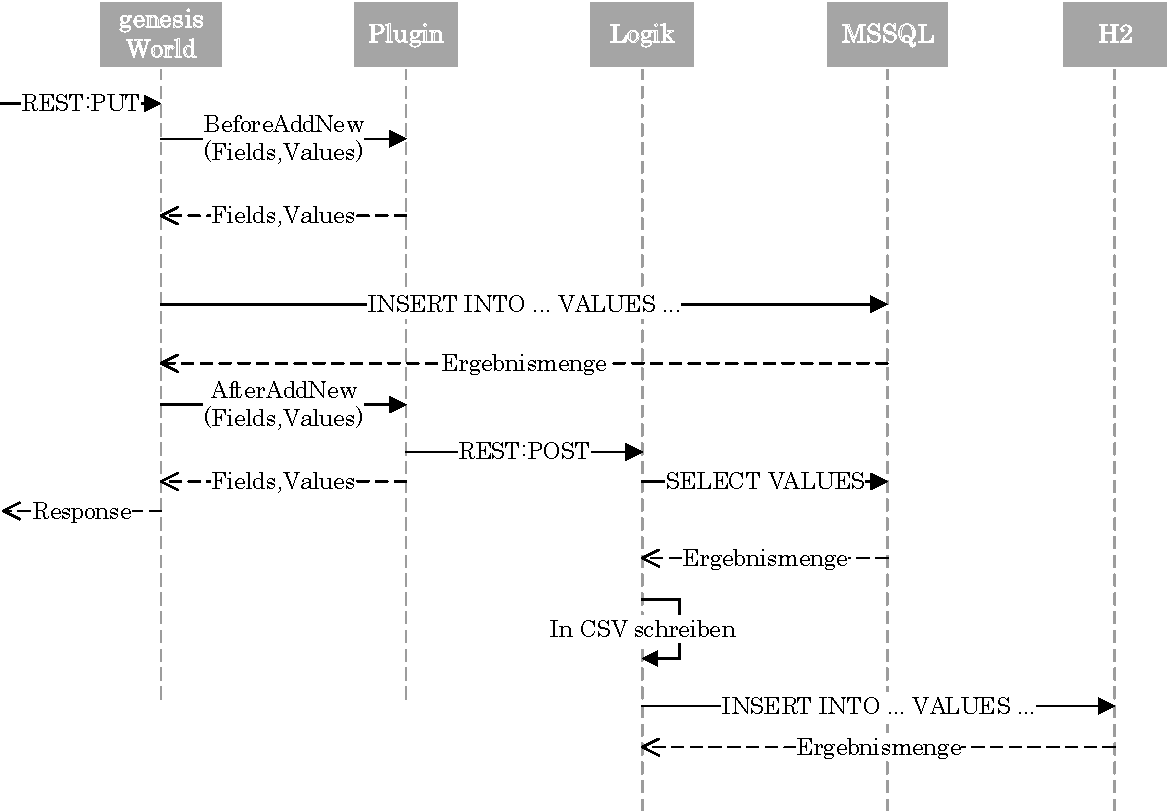
\includegraphics[width=1.0\textwidth, width=1.0\textwidth]{pics/sequenzdiagramm.pdf}
\caption{Sequenzdiagramm eines Updates}
\label{konzept_sequenz}
\end{figure}

In CAS genesisWorld gibt es eine Möglichkeit den zweiten Ansatz umzusetzen. Die Idee dabei ist den Applikationsserver um ein sogenanntes Plugin zu erweitern, dass über Veränderungen in den Datensätzen benachrichtigt wird. Realisiert wird ein solches Plugin als COM-Objekt, welches das Interface IGWSDKDataPlugIn implementiert. Das erstellte COM-Objekt wird im Server von CAS genesisWorld registriert. Der Server delegiert, wie in Abbildung \ref{konzept_sequenz} zu sehen, bei einer Datenoperation, den Aufruf an die für den jeweiligen Datensatz-Typen registrierten PlugIns. Das Plugin selbst besitzt einen REST-Client, der einen POST an die Logik sendet. Sie enthält die GGUID des Veränderten Datensatzes. Mithilfe dessen die Extraktion des betroffenen Datensatzes durchgeführt wird. Der neue Datensatz wird zuerst in einer CSV-Datei zwischengespeichert und anschließend in die H2-Datenbank eingefügt. Bei Updates werden die Datensätze einfach aktualisiert. 

%% ===========================
\section{Darstellungskonzepte}
\label{ch:Konzeption:sec:Darstellungskonzepte}
%% ===========================

Bei der Konzeption einer Darstellung, ist die Grad der Granularität von Informationen ein wichtiger Leitfaktor zur Bestimmung des Aufbaus. In unserem Fall ist nicht die Eigenschaft eines Verbindungsmerkmals von interessiere, sondern ihr Typ und ihre Häufigkeit zu einer bestimmten Person. Da keine Detailinformationen zum Verbindungsmerkmal vorhanden sind, kann jeder Benutzer frei wählen von welcher Person ausgehend, die Analyse stattfinden soll. Für die Oberfläche bedeutet dies einen Einstiegspunkt in Form eines Fensters, in dem der jeweilige Benutzername von dem die Suche ausgehen soll, eingegeben wird. Zusätzlich sollen die IP-Adresse und Portnummer des Server angebbar sein, falls dieser auf einem anderen Rechner läuft.

Nach dem Login findet eine Weiterleitung auf die eigentliche Seite statt. Dessen Aufbau ist in Abbildung \ref{konzept_darstellung} (a) zu sehen. Oben auf der Seite sind alle Regler, CheckBoxen und Eingabefelder zur Filterung der Ergebnismenge zu finden. Direkt darunter befindet sich das Diagramm das die Ergebnismenge einer Abfrage darstellt.

\begin{figure}[htbp]
\subfigure[Grober Entwurf des Aufbaus der Hauptseite]{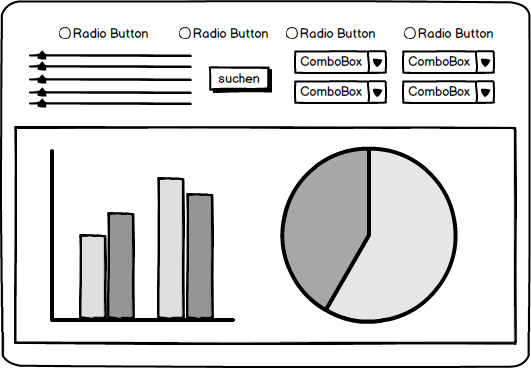
\includegraphics[width=0.49\textwidth]{pics/konzept_mockup.png}}\hfill
\subfigure[Tortendiagramm]{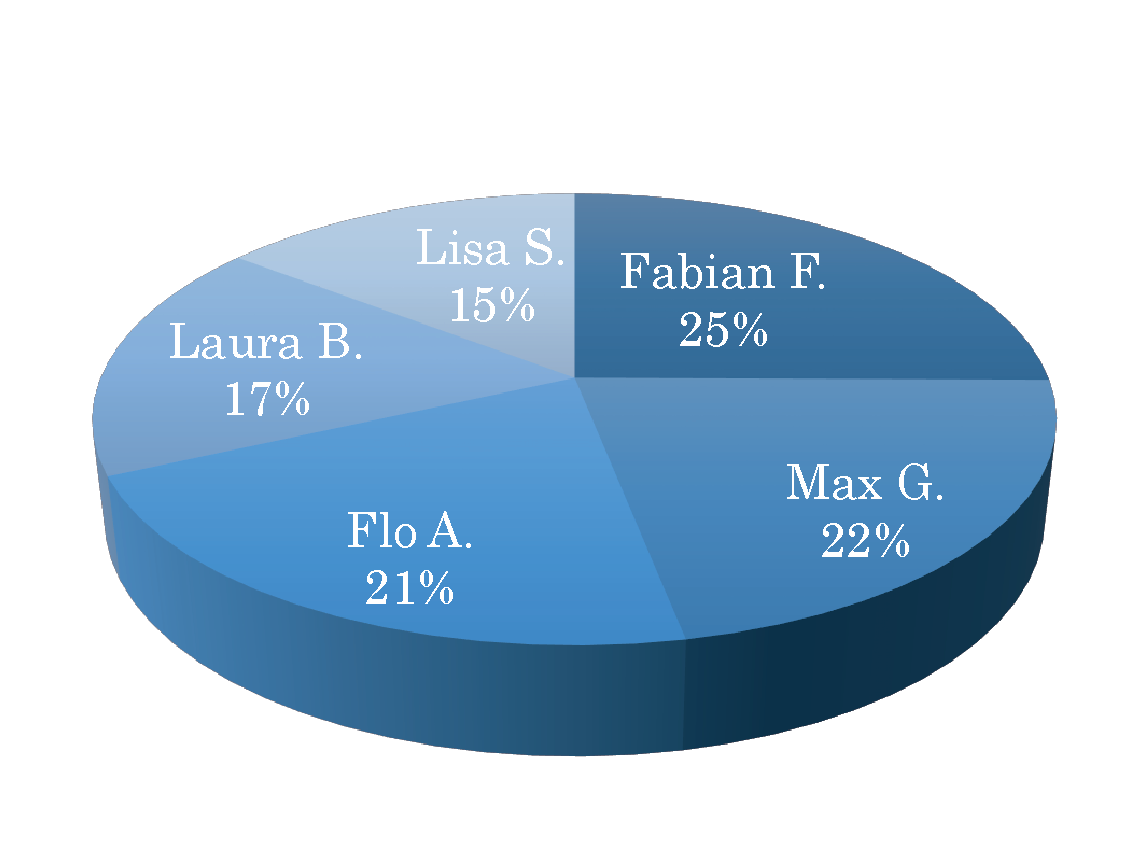
\includegraphics[width=0.49\textwidth]{pics/konzept_tortendiagramm.pdf}}\hfill
\subfigure[Balkendiagramm]{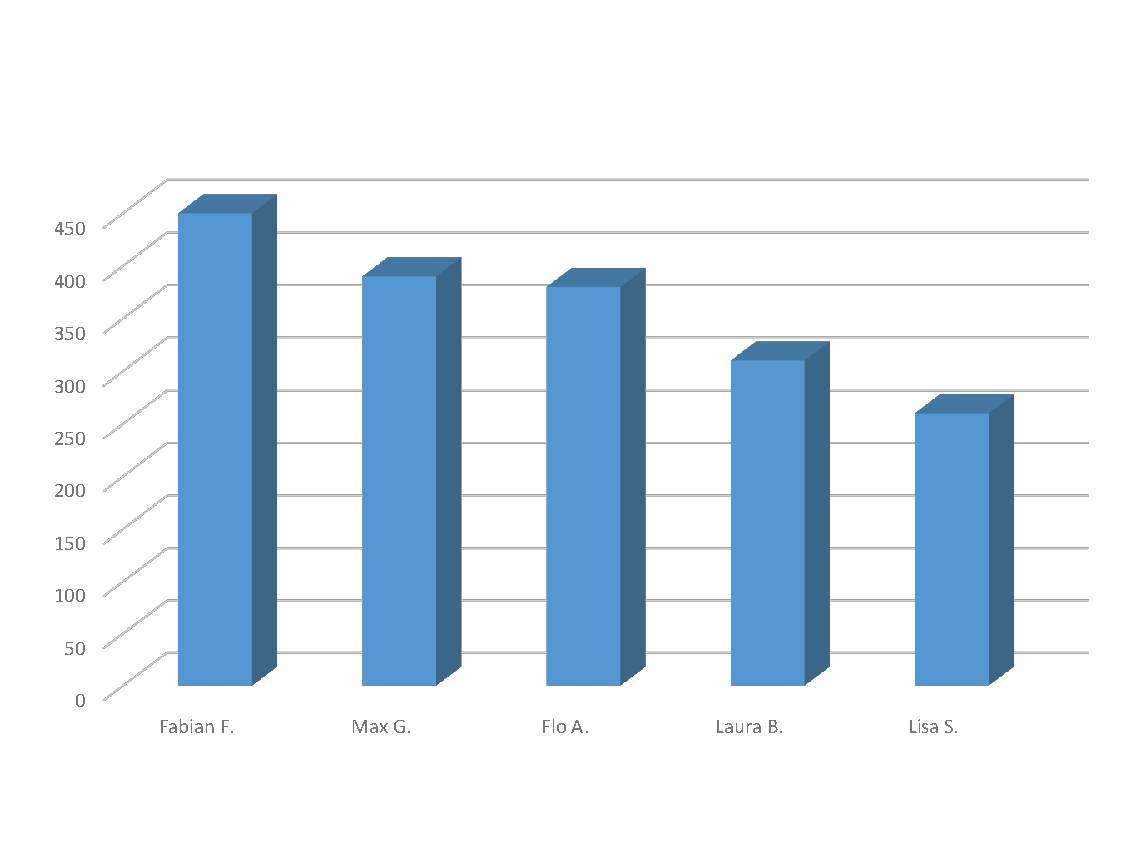
\includegraphics[width=0.49\textwidth]{pics/konzept_balkendiagramm.pdf}}\hfill
\subfigure[Tree Map]{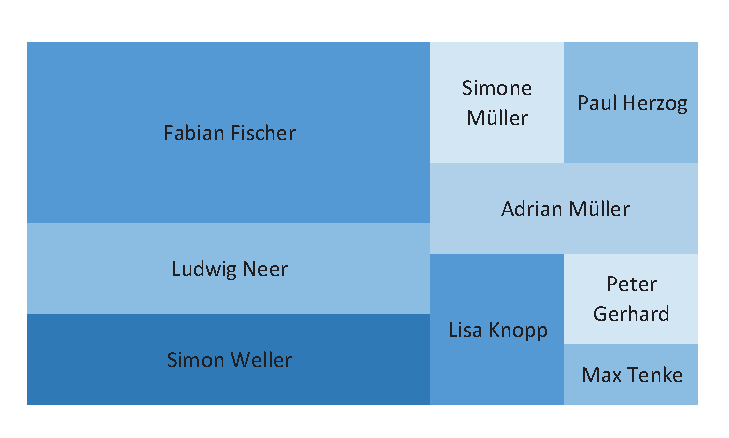
\includegraphics[width=0.49\textwidth]{pics/konzept_tree_map.pdf}}\hfill
\subfigure[Liniendiagramm]{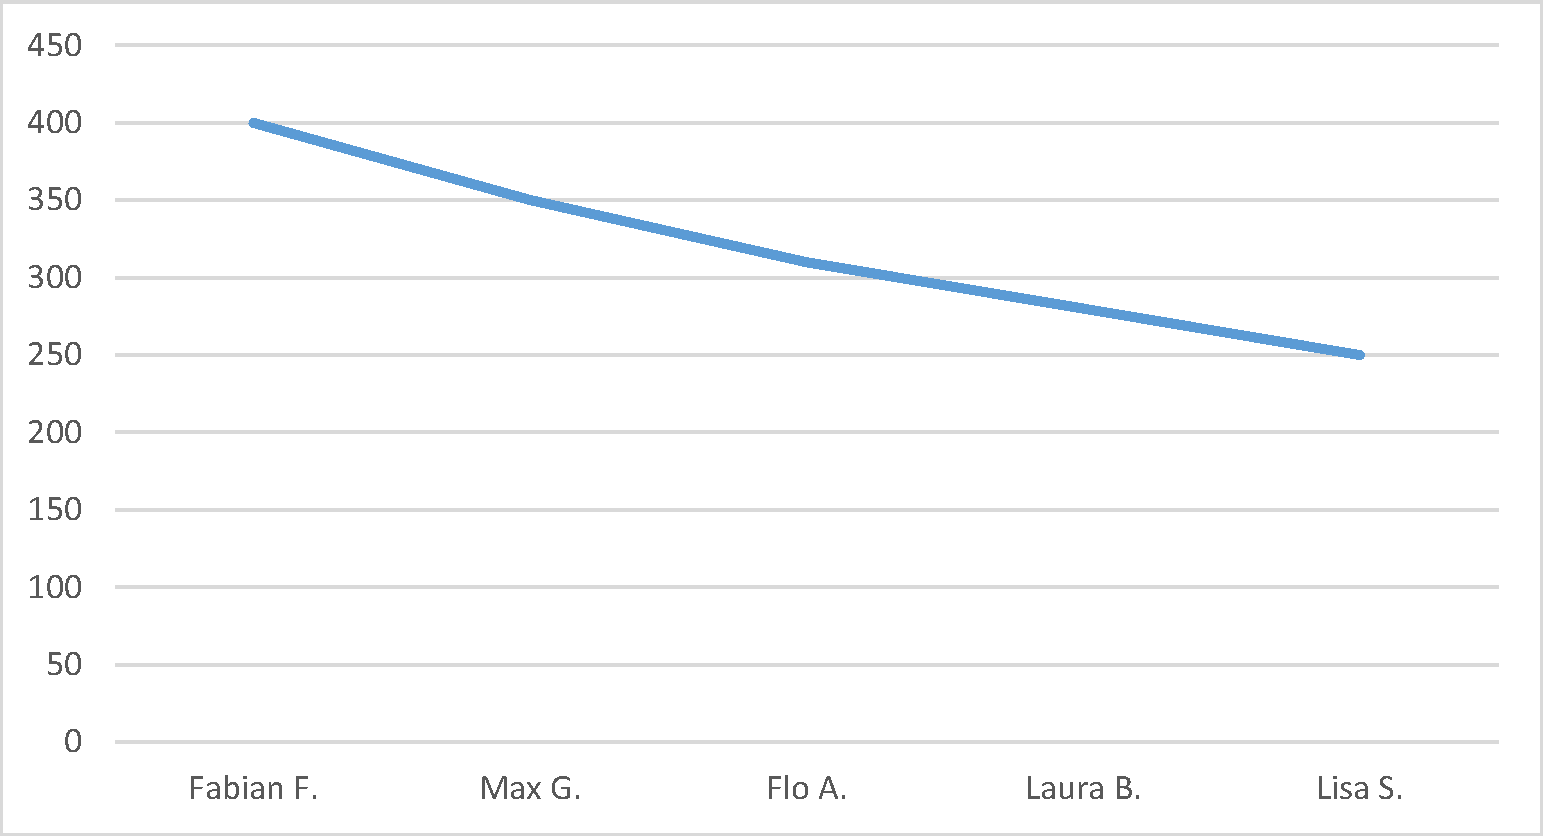
\includegraphics[width=0.49\textwidth]{pics/konzept_liniendiagramm.pdf}}\hfill
\subfigure[Netzdiagramm]{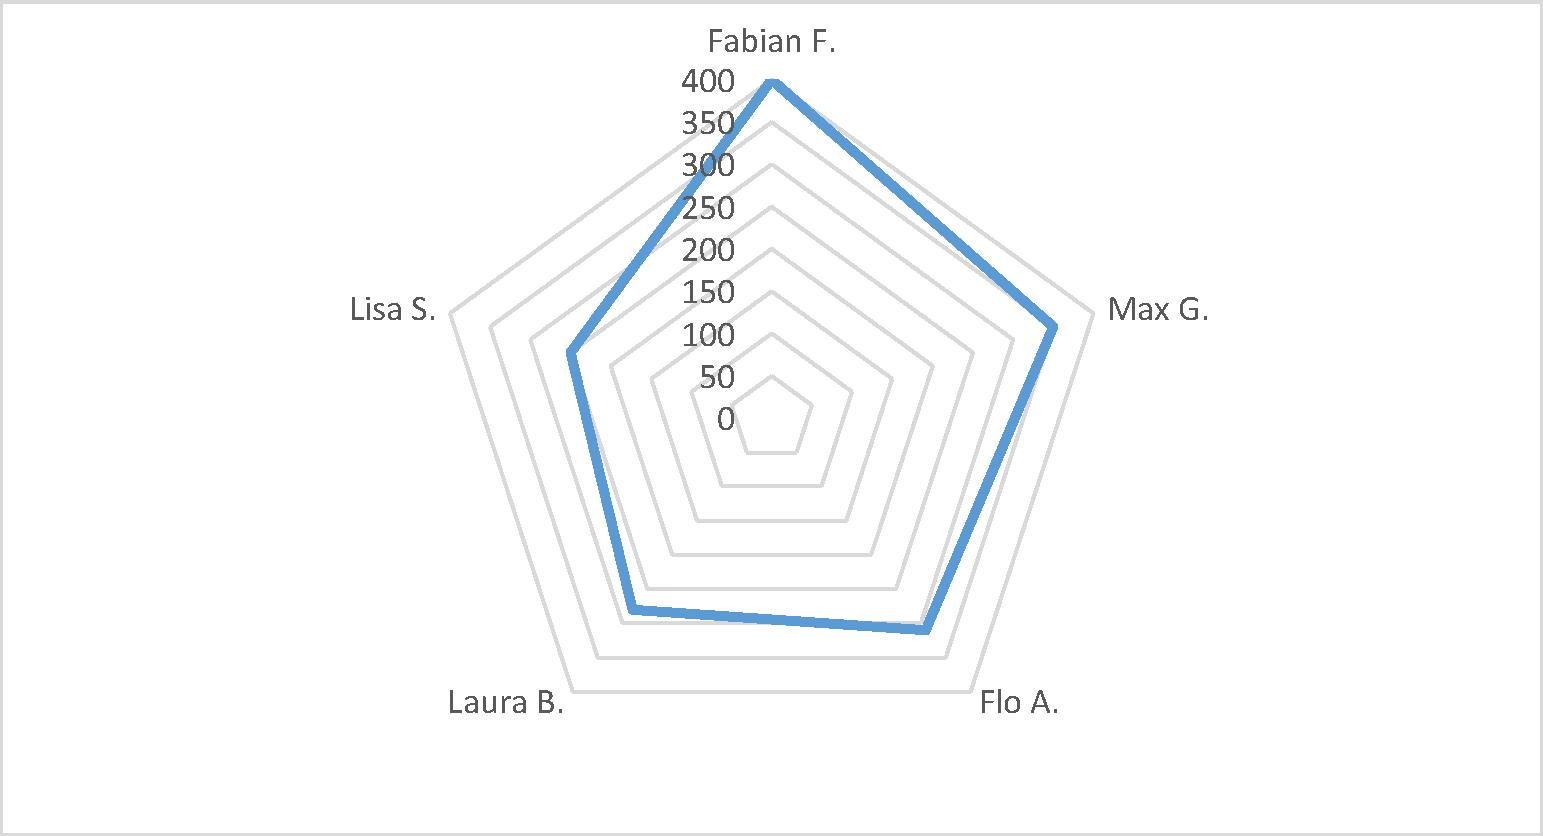
\includegraphics[width=0.49\textwidth]{pics/konzept_netzdiagramm.pdf}}
\caption{Entwürfe der Oberfläche}
\label{konzept_darstellung}
\end{figure}

Diagrammtypen gibt es viele jedoch ergeben sich Einschränkungen durch das Framework, welches zu Realisierung verwendet wird. Im Prinzip lässt sich jede Darstellung verwirklichen, allerdings ist das Aufwand Nutzen Verhältnis zu berücksichtigen. In einer Vorauswahl wurden einige Typen ausgewählt die in Abbildung \ref{konzept_darstellung} (b)-(f) dargestellt sind. 


Netzdiagramme geben Eigenschaften verschiedener Systeme wieder. Sie eignen sich daher gut zur Darstellung von Ausprägungen. Für unsere Form der Daten ist diese Darstellung gänzlich ungeeignet. Mithilfe von Liniendiagrammen lassen sich Trends und Zeitreihen darstellen. Die Verwendung verschiedener Linien ermöglicht zudem, die Darstellung mehrerer Trends. Die Benutzung dieses Diagramms macht keinen Sinn, da die Ergebnismenge sich nicht auf verschiedene Zeitpunkte bezieht, sondern die Summe der Werte in der Zeitreihe beinhaltet. Eine Tree Map dient der Abbildung von hierarchischen Daten. Dabei steht jede Fläche eines Rechtecks im proportionalen Zusammenhang zur Gesamtfläche. Die Beachtung von Größenverhältnissen stellt einen nützliche Eigenschaft für unsere Daten dar. Eine Hierarchie innerhalb der Daten ist nicht im klassischen Sinn vorhanden. Vielmehr würde jedes Rechteck aus dem jeweiligen Anteilen der Verbindungsmerkmale bestehen. Beispielweise könnte die Person Ludwig Neer wiederum in Rechtecke unterteilt werden, die die Anzahl der  Verbindungsmerkmale enthalten. Das würde allerdings schnell zu einer schlechten Übersicht führen, da viel zu viele Kacheln dargestellt werden müssen. Kreisdiagramme ermöglichen eine Betrachtung der Gesamtheit zu ihren Einzelstücken, da der Kreis ein geschlossenes System darstellt. Allerdings müssen alle Teile sich auf die gleiche Basis beziehen. Es eignet sich hervorragend zur Darstellung von Verhältnissen. Möchte man jedoch noch die Zusammenstellung eines einzelnen Stückes noch einmal aufteilen, ist ein zweite Ansicht nötig. Am besten dürfte sich ein Balkendiagramm eignen. Reihenfolgen beispielsweise lasse sich durch die resultierenden Stufen sehr gut darstellen. Balken selbst lassen sich außerdem in einzelne Teile aufspalten, ohne die Übersichtlichkeit zu verringern. Gegenüber dem Kreisdiagramm kann es zwar keine Betrachtung des Gesamten liefern ,allerdings ist das in diesem Anwendungsfall auch nicht nötig. 